\documentclass[lang=cn,10pt]{elegantbook}
\usepackage{subcaption}


\newcommand\bv[1]{\boldsymbol{#1}}
\newcommand\mb[1]{\mathbb{#1}}
\newcommand\mc[1]{\mathcal{#1}}

\title{大创参考文献学习笔记}
% \subtitle{Elegant\LaTeX{} 经典之作}

\author{Lollins}
% \institute{Elegant\LaTeX{} Program}
\date{\today}
% \version{4.3}
% \bioinfo{自定义}{信息}

\extrainfo{改变人生的事情,你必须冒险;
	意义非凡的事情,大多碰巧发生;
	不重要的事,才有周全的计划。
}

\setcounter{tocdepth}{3}

\cover{star.jpg}

\logo{logo.jpg}

% 本文档命令
\usepackage{array}
\newcommand{\ccr}[1]{\makecell{{\color{#1}\rule{1cm}{1cm}}}}

% 修改标题页的橙色带
\definecolor{customcolor}{RGB}{135, 206, 235}
\colorlet{coverlinecolor}{customcolor}

\begin{document}

\maketitle

\pagenumbering{roman}
\setcounter{page}{1}

\begin{center}
	\Huge\textbf{前言}
\end{center}
\par
$2023/8/14$,开始阅读老师给的三篇英文文献,用此文补充一些看大创文献中遇到的知识点。

$2023/9/19$,过去一个月了,最近在网上看到了Elegant\TeX 的模板,感觉好好看,花了一天的时间
把相关的格式和细节都改了。好看了好多,不过字体变小了不少。

\begin{flushright}
	\begin{tabular}{c}
		Lollins \\
		\today
	\end{tabular}
\end{flushright}

\newpage
\tableofcontents
\newpage

\chapter{Matrix Theorem}

\section{Laplace Matrix}
\subsection*{Laplace Operator}
\par 对于多元函数$f(x_1,...,x_n)$的Laplace Operator为
\begin{equation}
	\Delta f=\sum_{i=1}^n\frac{\partial^2f}{\partial x_i^2}
\end{equation}
\begin{example}
	三元函数$f(x,y,z)$的Laplace Operator为
	$$
		\Delta f=\frac{\partial^2f}{\partial x^2} + \frac{\partial^2f}{\partial y^2} + \frac{\partial^2f}{\partial z^2}
	$$
\end{example}

\subsection*{数值微分}
\par 根据导数近似计算公式,当$\Delta$近似等于$0$时,我们可以得到$f$的导数为
\begin{equation*}
	f'(x)\approx \frac{f(x+\Delta x) - f(x)}{\Delta x}
\end{equation*}
\begin{equation*}
	\begin{aligned}
		f''(x) & \approx \frac{f'(x+\Delta x) - f'(x)}{\Delta x}                    \\
		       & \approx \frac{f(x+\Delta x) + f(x-\Delta x) - 2f(x)}{(\Delta x)^2}
	\end{aligned}
\end{equation*}

\par 对二元函数$f(x,y)$,我们对其使用Laplace Operator,得到
\begin{equation*}
	\begin{aligned}
		\Delta f & =\frac{\partial^2f}{\partial x^2}+\frac{\partial^2f}{\partial y^2}                                                                                                                                                                                                                                                                                                                                                                                                                                                                                                                                                                                                                                                                                                                                   \\
		         & \begin{aligned}                                                                                                                                                                                                                                                                                                                                                                                                                                                                                                                                                                                                                                                                    & \approx\frac{f\left(x+\Delta x,y\right)+f\left(x-\Delta x,y\right)-2f\left(x,y\right)}{\left(\Delta x\right)^2}
                                                                                                                                                                                                                                                                                                                                                                                                                                                                                                                                                                                                                                                                                  \\&+\frac{f\left(x,y+\Delta y\right)+f\left(x,y-\Delta y\right)-2f\left(x,y\right)}{\left(\Delta y\right)^2}\end{aligned}
	\end{aligned}
\end{equation*}
\par 把此二元函数离散化,为了简化,假设$x$和$y$的增量即步长为$1$,即
$$
	\Delta x =x_{i+1} - x_i=1, \Delta y =y_{j+1} - y_j=1
$$
\par 点$(x_i, y_j)$处的Laplace Operator可以用下面的公式近似代替
\begin{equation*}
	\begin{aligned}
		  & \frac{f\left(x_i+\Delta x,y_j\right)+f\left(x_i-\Delta x,y_j\right)-2f\left(x_i,y_j\right)}{\left(\Delta x\right)^2}
		\\&+\frac{f\left(x_i,y_j+\Delta y\right)+f\left(x_i,y_j-\Delta y\right)-2f\left(x_i,y_j\right)}{\left(\Delta y\right)^2}                                                             \\
		= & \frac{f\left(x_{i+1},y_j\right)+f\left(x_{i-1},y_j\right)-2f\left(x_i,y_j\right)}{1^2}+\frac{f\left(x_i,y_{j+1}\right)+f\left(x_i,y_{j-1}\right)-2f\left(x_i,y_j\right)}{1^2} \\
		= & f\left(x_{i+1},y_j\right)+f\left(x_{i-1},y_j\right)+f\left(x_i,y_{j+1}\right)+f\left(x_i,y_{j-1}\right)-4f\left(x_i,y_j\right)
	\end{aligned}
\end{equation*}
\par 这是非常优美的结果,它就是$(x_i,y_j)$的$4$个相邻点处的函数值
之和与$4$倍的$(x_i,y_j)$点处的差值,如图\ref{aj}所示

\begin{figure}[h]
	\centering
	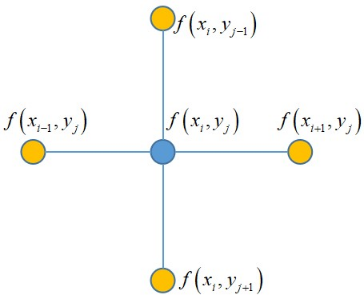
\includegraphics[width = 8cm]{img/aj.png}
	\caption{}
	\label{aj}
\end{figure}
\par 基于这种表示,Laplace Operator的计算公式可以表示为
\begin{equation}
	\begin{aligned}
		\Delta f & =f\left(x_{i+1},y_j\right)+f\left(x_{i-1},y_j\right)+f\left(x_i,y_{j+1}\right)+f\left(x_i,y_{j-1}\right)-4f\left(x_i,y_j\right) \\
		         & =f\left(x_{i+1},y_j\right)-f\left(x_i,y_j\right)+f\left(x_{i-1},y_j\right)-f\left(x_i,y_j\right)                                \\
		         & +f\left(x_i,y_{j+1}\right)-f\left(x_i,y_j\right)+f\left(x_i,y_{j-1}\right)-f\left(x_i,y_j\right)                                \\
		         & =\sum_{(k,l)\in N(i,j)}\left(f\left(x_k,y_l\right)-f\left(x_i,y_j\right)\right)
	\end{aligned}
\end{equation}
\par 其中$N(i,j)$为$(x_i,y_j)$的邻居节点
\subsection*{图的邻接矩阵与加权度矩阵}
\par 图是一种几何结构,对它的研究起源于古老的哥尼斯堡七桥问题。
一个图$G(graph)$由顶点和边构成,通常将顶点的集合记为$V(vertex)$,
边的集合记为$E(edge)$。边由其连接的起点和终点表示。如图\ref{g}所示,
它是一个典型的图。
\begin{figure}[h]
	\centering
	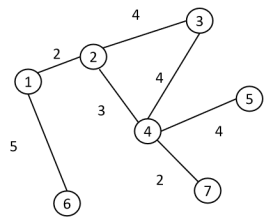
\includegraphics[scale = 0.8]{img/g.png}
	\caption{}
	\label{g}
\end{figure}
\par 图的边可以是有方向的,也可以是无方向的,前者被称为有向图,
后者被称为无向图。邻接矩阵是用来方便存储图的结构,用线性代数的方法
研究图的问题。
\par 如果一个图有$n$个顶点,其邻接矩阵$W$为$n \times n$的
矩阵,矩阵元素$w_{ij}$表示边$(i,j)$的权重,如果矩阵两个顶点
之间没有边连接,则记为$0$。对于无向连接矩阵,满足$w_{ij} = w_{ji}$。图\ref{g}的邻接
矩阵如下
\begin{equation*}
	\begin{bmatrix}
		0 & 2 & 0 & 0 & 0 & 5 & 0 \\
		2 & 0 & 4 & 3 & 0 & 0 & 0 \\
		0 & 4 & 0 & 4 & 0 & 0 & 0 \\
		0 & 3 & 4 & 0 & 4 & 0 & 2 \\
		0 & 0 & 0 & 4 & 0 & 0 & 0 \\
		5 & 0 & 0 & 0 & 0 & 0 & 0 \\
		0 & 0 & 0 & 2 & 0 & 0 & 0
	\end{bmatrix}
\end{equation*}
\par 对于无向图,顶点的加权度是与该顶点相关的所有边的权重之和。
对于无向图连接矩阵$W$,顶点$i$的加权度为$W$第$i$行元素之和
\begin{equation*}
	d_i = \sum_{j=1}^nw_{ij}
\end{equation*}
\par 加权度矩阵$D$为对角矩阵,其主对角线元素为每个顶点的加权度,其他位置的元素为$0$。
\begin{equation}
	d_{ii} = d_i = \sum_{j=1}^nw_{ij}
\end{equation}
\par 对于图\ref{g},它的加权度矩阵如式\ref{eq1.4}所示

\begin{equation} \label{eq1.4}
	\begin{bmatrix}
		7 & 0 & 0 & 0  & 0 & 0 & 0 \\
		0 & 9 & 0 & 0  & 0 & 0 & 0 \\
		0 & 0 & 8 & 0  & 0 & 0 & 0 \\
		0 & 0 & 0 & 13 & 0 & 0 & 0 \\
		0 & 0 & 0 & 0  & 4 & 0 & 0 \\
		0 & 0 & 0 & 0  & 0 & 5 & 0 \\
		0 & 0 & 0 & 0  & 0 & 0 & 2
	\end{bmatrix}
\end{equation}
\subsection*{Laplace Matrix}
\par 如果将图的顶点处的值看作是函数值,则在顶点$i$处的
Laplace Operator为
\begin{equation*}
	\Delta f_i=\sum_{j\in N_i}\left(f_i-f_j\right)
\end{equation*}
\par 这里的$N_i$为顶点$i$的所有邻居顶点集合。这里我们调换了
$f_i$和$f_j$的位置,和之前的Laplace Operator相比,相当于多了一个负号。
由于图的边可以带有权重,我们可以在上面的计算公式中加上权重
\begin{equation} \label{eq1.5}
	\Delta f_i=\sum_{j\in N_i}w_{ij}\left(f_i-f_j\right)
\end{equation}
\par 这一推广如图\ref{tg}所示,图中图中红色的顶点是$i$,
蓝色的顶点是它的邻居顶点,灰色的顶点是其他顶点。
\par 如果$j$不是$i$的邻居,则$w_{ij}=0$。因此式\ref{eq1.5}也可以写做
\begin{equation}
	\Delta f_i=\sum_{j\in N_i}w_{ij}\left(f_i-f_j\right)=\sum_{j\in N_i}w_{ij}f_i-\sum_{j\in N_i}w_{ij}f_j=d_if_i-\mathbf{w}_i\mathbf{f}
\end{equation}
\par 这里的$d_i$就是第$i$个节点的加权度,$\bv{w_i}$为邻接矩阵第$i$行,
$\bv{f}$是所有顶点的值构成的列向量,$\bv{w_if}$是二者的内积。
\begin{figure}[h]
	\centering
	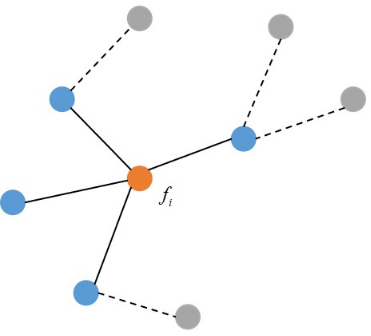
\includegraphics[scale=0.8]{img/tg.png}
	\caption{}
	\label{tg}
\end{figure}

对图的所有顶点,我们有
\begin{equation}
	\begin{aligned}
		\Delta f & =
		\begin{bmatrix}\Delta f_1\\...\\\Delta f_n\end{bmatrix}=\begin{bmatrix}d_1f_1-\mathbf{w}_1\mathbf{f}\\...\\d_nf_n-\mathbf{w}_n\mathbf{f}\end{bmatrix}=\begin{bmatrix}d_1&...&...\\...&...&...\\...&...&d_n\end{bmatrix}\begin{bmatrix}f_1\\...\\f_n\end{bmatrix}-\begin{bmatrix}\mathbf{w}_1\\...\\...\\\mathbf{w}_n\end{bmatrix}\begin{bmatrix}f_1\\...\\...\\f_n\end{bmatrix} \\
		         & =\left(\mathbf{D}-\mathbf{W}\right)\mathbf{f}
	\end{aligned}
\end{equation}
\par 我们在邻接矩阵和加权度矩阵的基础上定义Laplace Matrix。假设
无向图$G$有$n$个顶点,邻接矩阵为$W$,加权度矩阵为$D$。Laplace Matrix
定义为加权度矩阵与邻接矩阵之差,即
\begin{equation}
	L = D-W
\end{equation}
\par 则图\ref{g}的Laplace Matrix为
\begin{equation*}
	\begin{bmatrix}
		7 & 0 & 0 & 0  & 0 & 0 & 0 \\
		0 & 9 & 0 & 0  & 0 & 0 & 0 \\
		0 & 0 & 8 & 0  & 0 & 0 & 0 \\
		0 & 0 & 0 & 13 & 0 & 0 & 0 \\
		0 & 0 & 0 & 0  & 4 & 0 & 0 \\
		0 & 0 & 0 & 0  & 0 & 5 & 0 \\
	\end{bmatrix}-
	\begin{bmatrix}
		0 & 2 & 0 & 0 & 0 & 5 & 0 \\
		2 & 0 & 4 & 3 & 0 & 0 & 0 \\
		0 & 4 & 0 & 4 & 0 & 0 & 0 \\
		0 & 3 & 4 & 0 & 4 & 0 & 2 \\
		0 & 0 & 0 & 4 & 0 & 0 & 0 \\
		5 & 0 & 0 & 0 & 0 & 0 & 0 \\
		0 & 0 & 0 & 2 & 0 & 0 & 0
	\end{bmatrix}=
	\begin{bmatrix}
		7  & -2 & 0  & 0  & 0  & -5 & 0  \\
		-2 & 9  & -4 & -3 & 0  & 0  & 0  \\
		0  & -4 & 8  & -4 & 0  & 0  & 0  \\
		0  & -3 & -4 & 13 & -4 & 0  & -2 \\
		0  & 0  & 0  & -4 & 4  & 0  & 0  \\
		-5 & 0  & 0  & 0  & 0  & 5  & 0  \\
		0  & 0  & 0  & -2 & 0  & 0  & 2
	\end{bmatrix}
\end{equation*}
\par 显然Laplace Matrix的每行元素之和都为$0$。
\subsubsection*{Properties}
\textbf{$\mathit{1.}$}对任意向量$\bv{f} \in \mathbb{R}^n$,有
\begin{equation*}
	\mathbf{f}^\mathrm{T}\mathbf{L}\mathbf{f}=\frac12\sum_{i=1}^n\sum_{j=1}^nw_{ij}\left(f_i-f_j\right)^2
\end{equation*}

\textbf{$\mathit{2.}$}Laplace Matrix是对称半正定矩阵;

\textbf{$\mathit{3.}$}Laplace Matrix的最小特征值为$0$,其对应的特征向量为常向量
$1$,即所有分量为$1$,即$L\bv{1}_n = 0\bv{1}_n = \bv{0}_n$;

\textbf{$\mathit{4.}$}Laplace Matrix有$n$个非负实数特征值,并且满足
\begin{equation*}
	\lambda_n \ge \ldots \ge \lambda_1 \ge 0
\end{equation*}

相关证明可以参考这篇知乎文章
\href{https://zhuanlan.zhihu.com/p/362416124}{理解图的拉普拉斯矩阵}

\section{Kronecker Product}
\begin{definition}
	给定任意矩阵$X \in \mathbb{R}^{m \times n}$和$Y \in \mathbb{R}^{p \times q}$
	则矩阵$X$和$Y$的Kronecker Product为
	\begin{equation}\label{eq1.9}
		X\otimes Y = \begin{bmatrix}
			x_{11}\boldsymbol{Y} & x_{12}\boldsymbol{Y} & \cdots & x_{1n}\boldsymbol{Y} \\x_{21}\boldsymbol{Y}&x_{22}\boldsymbol{Y}&\cdots&x_{2n}\boldsymbol{Y}\\\vdots&\vdots&\ddots&\vdots\\x_{m1}\boldsymbol{Y}&x_{m2}\boldsymbol{Y}&\cdots&x_{mn}\boldsymbol{Y}
		\end{bmatrix}\in\mathbb{R}^{(mp)\times(nq)}
	\end{equation}
	其中,$\otimes$表示Kronecker Product。
\end{definition}
\textbf{注:}根据式\ref{eq1.9},我们可以得到
\begin{equation*}
	\boldsymbol{Y}\otimes\boldsymbol{X}=
	\begin{pmatrix}
		y_{11}\boldsymbol{X} & y_{12}\boldsymbol{X} & \cdots & y_{1q}\boldsymbol{X} \\
		y_{21}\boldsymbol{X} & y_{22}\boldsymbol{X} & \cdots & y_{2q}\boldsymbol{X} \\
		\vdots               & \vdots               & \ddots & \vdots               \\
		y_{p1}\boldsymbol{X} & y_{p2}\boldsymbol{X} & \cdots & y_{pq}\boldsymbol{X}
	\end{pmatrix}
	\in\mathbb{R}^{(mp)\times(nq)}
\end{equation*}
这意味着$\boldsymbol{X}\otimes\boldsymbol{Y}$和$\boldsymbol{Y}\otimes\boldsymbol{X}$
不相同,即Kronecker Product不存在交换律。

\subsection*{Properties}
\noindent
\textbf{$\mathit{1.}$结合律(associativity)}
\begin{equation}
	X\otimes Y\otimes Z=(X\otimes Y)\otimes Z=X\otimes(Y\otimes Z)
\end{equation}
\textbf{$\mathit{2.}$分配律(distributivity)}
\begin{equation}
	(\boldsymbol{X}+\boldsymbol{Y})\otimes\boldsymbol{Z}=\boldsymbol{X}\otimes\boldsymbol{Z}+\boldsymbol{Y}\otimes\boldsymbol{Z}
\end{equation}
\textbf{$\mathit{3.}$}给定任意矩阵$X \in \mathbb{R}^{m \times n}$和$Y \in \mathbb{R}^{p \times q}$,
则
\begin{equation}
	(X \otimes Y)^T = X^T \otimes Y^T
\end{equation}
\textbf{$\mathit{4.}$}给定任意矩阵$X\in \mathbb{R}^{m\times n}\text{、}Y\in \mathbb{R}^{s\times t}\text{、}U\in \mathbb{R}^{n\times p}$
和$V\in \mathbb{R}^{t\times q}$,则
\begin{equation}
	\left( X\otimes Y \right) \left( U\otimes V \right) =\left( XU \right) \otimes \left( YV \right) \in \mathbb{R}^{\left( ms \right) \times \left( pq \right)}
\end{equation}
\textbf{$\mathit{5.}$}给定矩阵$X \in \mathbb{R}^{m \times n}$和$Y \in \mathbb{R}^{p \times q}$
都是非奇异的,则
\begin{equation}
	(X \otimes Y)^{-1} = X^{-1} \otimes Y^{-1}
\end{equation}
\par 还有一些特殊性质(懒打公式了,先从网上找了图片截屏放进去),如图\ref{Kronecker}所示
\begin{figure}[h]
	\centering
	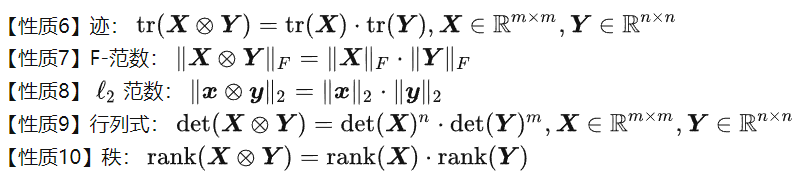
\includegraphics[scale=0.8]{img/Kronecker.png}
	\caption{}
	\label{Kronecker}
\end{figure}

本节主要参考了知乎的
\href{https://zhuanlan.zhihu.com/p/139335389}{代数基础 | Kronecker积},文章中给出了详细的证明。

\section{Frobenius Norm and Inner Product}
\begin{definition}
	对于矩阵$A \in C^{m \times n}$,其Frobenius Norm为
	\begin{equation}
		\|A\|_F = \left(\sum_{i=1}^m \sum_{j=1}^n |a_{ij}|^2\right)^{\frac{1}{2}}
	\end{equation}
	\par 其Frobenius Inner Product为
	\begin{equation}
		\langle A,B \rangle_F = \sum_{j=1}^m\sum_{i=1}^nA_{ij}^*B_{ij}
	\end{equation}
\end{definition}
又由于
\begin{equation*}
	\begin{aligned}
		tr(A^HB) & =\sum_{i=1}^n(A^HB)_{ii}                \\
		         & =\sum_{i=1}^n\sum_{k=1}^mA_{ik}^HB_{ki} \\
		         & =\sum_{i=1}^n\sum_{k=1}^mA_{ki}^*B_{ki}
	\end{aligned}
\end{equation*}

故我们可以得到
\begin{equation*}
	\langle A,B \rangle_F = tr(A^HB)
\end{equation*}

\par 本节主要参考了
\href{https://zhuanlan.zhihu.com/p/619586436}{Frobenius范数和内积的关系}

\section{Diagonally-dominant Matrix}
\begin{definition}[Strictly Diagonally-dominant Matrix]
	对于一个矩阵$A_{n \times n}$,满足$\forall i = 1,2\ldots,n$,有
	\begin{equation}
		|a_{ii}|>\sum_{j\neq i}|a_{ij}|
	\end{equation}
	\par 那么我们称$A_{n \times n}$为Strictly Diagonally-dominant Matrix。
\end{definition}

\begin{theorem}
	如果矩阵A严格对角占优,则A非奇异。
\end{theorem}

具体的证明可以参考这篇文章\href{https://zhuanlan.zhihu.com/p/512029879}{严格对角占优矩阵非奇异}。

\section{Hurwitz Matrix}
\begin{definition}[Hurwitz Matrix]\label{de1.5}
	给定一个多项式(多项式的所有根都有负实部)
	\begin{equation}
		p(z)=a_{n}z^{n}+a_{n-1}z^{n-1}+\cdots+a_{1}z+a_{0}
	\end{equation}
	和n阶矩阵
	\begin{equation}
		H=
		\begin{pmatrix}
			a_{n-1} & a_{n-3} & a_{n-5} & \ldots & \ldots & \ldots & 0      & 0      & 0      \\
			a_n     & a_{n-2} & a_{n-4} &        &        &        & \vdots & \vdots & \vdots \\
			0       & a_{n-1} & a_{n-3} &        &        &        & \vdots & \vdots & \vdots \\
			\vdots  & a_n     & a_{n-2} & \ddots &        &        & 0      & \vdots & \vdots \\
			\vdots  & 0       & a_{n-1} &        & \ddots &        & a_0    & \vdots & \vdots \\
			\vdots  & \vdots  & a_n     &        &        & \ddots & a_{1}  & 0      & \vdots \\
			\vdots  & \vdots  & 0       &        &        &        & a_{2}  & a_0    & \vdots \\
			\vdots  & \vdots  & \vdots  &        &        &        & a_{3}  & a_{1}  & 0      \\
			0       & 0       & 0       & \cdots & \cdots & \cdots & a_{4}  & a_{2}  & a_0
		\end{pmatrix}
	\end{equation}
	\par 那么称矩阵H为多项式p的Hurwitz Matrix。

	p多项式的所有根都有负实部 $\Longleftrightarrow$ H的所有顺序主子式大于0。
\end{definition}

\begin{example}
	在Mathematica中调用函数指令,可以得到$p(x)=5+4x+3x^2$
	和$p(x)=5+4x+3x^2+2x^3+x^4$的2阶与4阶的
	Hurwitz Matrix,分别如图\ref{hurwitz1}和图\ref{hurwitz2}
	所示(原本想\LaTeX 嵌入mma代码,奈何网上资料太少加上自己能力有限,嵌入失败,就截图放里面了)
	\begin{figure}[h]
		\centering
		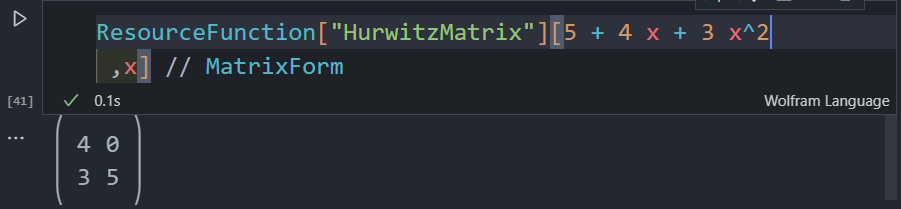
\includegraphics[scale=0.6]{img/hurwitz1.png}
		\caption{}
		\label{hurwitz1}
	\end{figure}
	\begin{figure}[h]
		\centering
		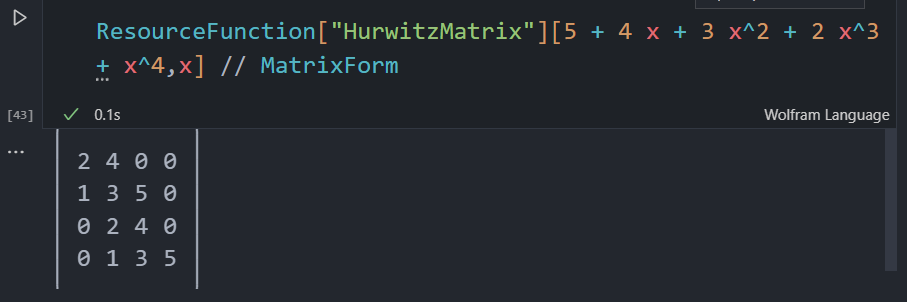
\includegraphics[scale=0.6]{img/hurwitz2.png}
		\caption{}
		\label{hurwitz2}
	\end{figure}
\end{example}

\begin{theorem}
	求解n阶方阵的全部顺序主子式$D_i$,$D_i$表示矩阵的第$i$阶主子式。
	\begin{enumerate}
		\item 如果所有主子式$D_i$均为正,则系统稳定;
		\item 如果存在某个主子式$D_i$为零,但其后续主子式均为正,则系统稳定;
		\item 如果任意一个主子式$D_i$为负,则系统不稳定。
	\end{enumerate}
\end{theorem}


\chapter{Convex Optimization}
\section{Convex Function}
\subsection*{基本的定义与性质}
\begin{definition}[Convex Function]
	对于函数${f}:\mathbb{R}^n \to \mathbb{R}$,若满足$dom( {f}) \subset \mb{R}^n$
	是凸集,$\forall t \in [0,1]$,$\forall \bv{x,y} \in dom( {f})$,有
	\begin{equation}
		f(t\bv{x}+(1-t)\bv{y})\leq tf(\bv{x})+(1-t)f(\bv{y})
	\end{equation}

	则这个函数是一个凸函数。如果等号处处不成立,则称它是一个严格凸函数(Strictly)。
\end{definition}
\begin{definition}[Concave Functions]
	若$-f$是一个凸函数,那么$f$所定义的函数就是凹函数。如果等号处处不成立,则称它是一个严格凹函数。
\end{definition}

\textbf{注1:}凸函数与凹函数不是二元对立的关系,比如$y=ax+b,x \in \mb{R}$,它是凸函数也是凹函数

\textbf{注2:}无论是凸函数,还是凹函数,一定要求定义域为凸集。而且没有凹集的说法

\begin{definition}[First-order Characterization of Convex Functions]
	\label{de2.1.3}
	如果$f$一阶可导,$dom(f)$是凸的,并且$\forall \bv{x,y} \in dom(f)$,有
	\begin{equation}\label{eq2.2}
		f(\bv{y}) \geq f(\bv{x}) + \nabla f(\bv{x})^T (\bv{y-x})
	\end{equation}

	则称它是一个凸函数。
\end{definition}

其实定义\ref{de2.1.3}可以看成$Taylor$公式的一阶展开。

\begin{figure}[h]
	\centering
	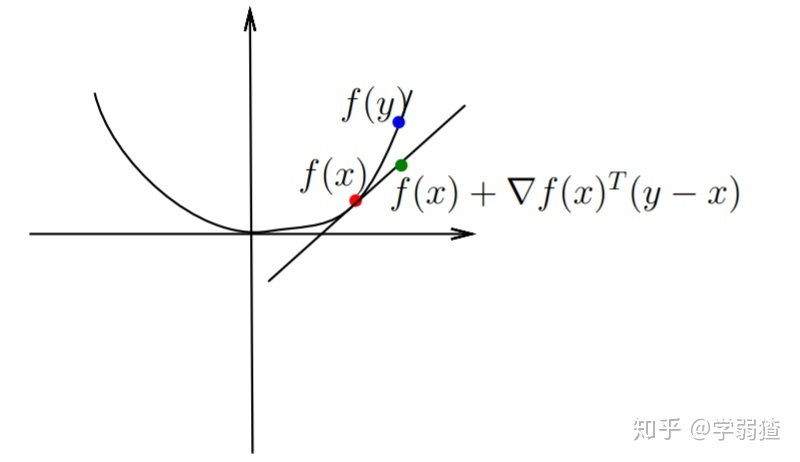
\includegraphics[scale = 0.5]{img/cf3.jpg}
	\caption{}
	\label{cf3}
\end{figure}

对于这个一阶条件定义,可以参照图\ref{cf3}来理解。

它给了我们一个重要的启示:如果我们假设$\nabla f(\bv{x})=0$,那么无论$\bv{y}$
是什么,都有$f(\bv{y}) \geq f(\bv{x})$。潜在的意思是,对于驻点为$0$的$\bv{x}$点,
我们取到了最小值。因此正如机器学习界经常说的一句话:\textbf{当一个问题被证明是一个凸优化问题,那么基本上就可以算解决了}。

\begin{definition}[Second-order Characterization of Convex Functions]
	如果$f$是二阶可微的,$dom(f)$是凸的,并且$\forall x \in dom(f),\nabla^2f(x)\succeq 0$。
	那么f就是一个凸函数。
\end{definition}
二阶导数(即$\nabla^2 f$)是用来衡量一阶导数的变化率。考虑$dom(f) \subset \mb{R}$的一维情况,对应$\nabla^2 f \geq 0$
画出$\nabla f$图像的三种情况,如图\ref{cf41}所示,
对应的$f$图像如\ref{cf42}所示,我们可以发现图\ref{cf42}都为凸函数。

\begin{figure}[h]
	\centering
	\begin{subfigure}{0.4\linewidth}
		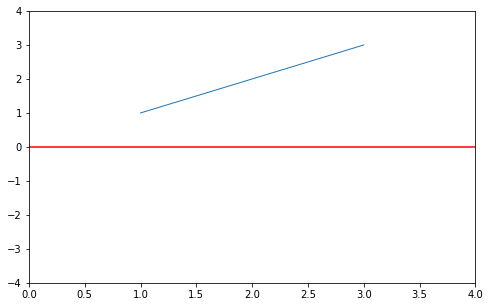
\includegraphics[width=\linewidth]{img/cf4_1.png}
		\caption{$\nabla f$在$x$轴上方}
		\label{cf4_1}
	\end{subfigure}
	\hspace{0.5in} % 两图片之间的距离
	\begin{subfigure}{0.4\linewidth}
		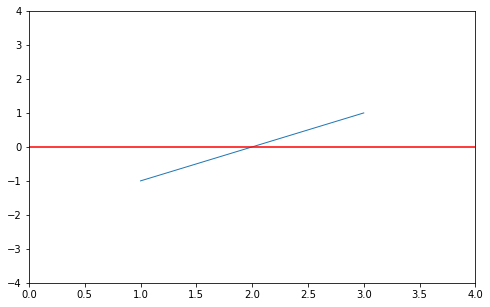
\includegraphics[width=\linewidth]{img/cf4_2.png}
		\caption{$\nabla f$穿过$x$轴}
		\label{cf4_2}
	\end{subfigure}
	\hspace{0.5in} % 两图片之间的距离
	\begin{subfigure}{0.4\linewidth}
		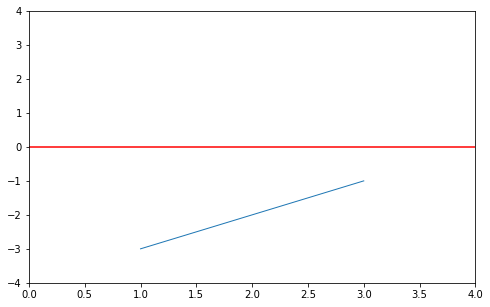
\includegraphics[width=\linewidth]{img/cf4_3.png}
		\caption{$\nabla f$在$x$轴下方}
		\label{cf4_3}
	\end{subfigure}
	\caption{$\nabla f$图像的三种情况}
	\label{cf41}
\end{figure}

\begin{figure}[h]
	\centering
	\begin{subfigure}{0.4\linewidth}
		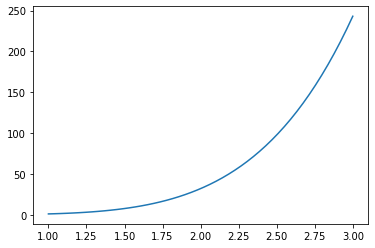
\includegraphics[width=\linewidth]{img/cf4_4.png}
		\caption{对应$\nabla f$在$x$轴上方}
		\label{cf4_4}
	\end{subfigure}
	\hspace{0.5in} % 两图片之间的距离
	\begin{subfigure}{0.4\linewidth}
		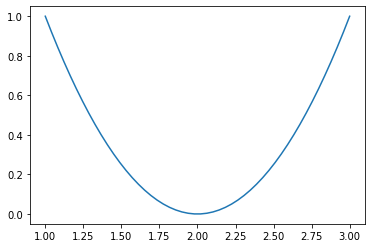
\includegraphics[width=\linewidth]{img/cf4_5.png}
		\caption{对应$\nabla f$穿过$x$轴}
		\label{cf4_5}
	\end{subfigure}
	\hspace{0.5in} % 两图片之间的距离
	\begin{subfigure}{0.4\linewidth}
		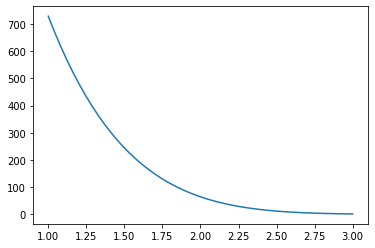
\includegraphics[width=\linewidth]{img/cf4_6.png}
		\caption{对应$\nabla f$在$x$轴下方}
		\label{cf4_6}
	\end{subfigure}
	\caption{$f$图像的三种情况}
	\label{cf42}
\end{figure}

\begin{corollary}
	如果f是凸函数,那么$\forall \bv{x,y}$,我们有
	\begin{equation}
		(\nabla f(\bv{x}) - \nabla f(\bv{y}))^T (\bv{x-y}) \geq 0
	\end{equation}
\end{corollary}

\begin{proof}
	\textbf{1、}从一维的角度理解,$\nabla^2 f \geq 0 \Rightarrow \nabla f$为增函数,即证!

	\textbf{2、}根据公式\ref{eq2.2},我们有
	\begin{equation*}
		\begin{cases}
			\begin{aligned}
				f(\bv{y}) & \geq f(\bv{x}) + \nabla f(\bv{x})^T (\bv{y-x}) \\
				f(\bv{x}) & \geq f(\bv{y}) + \nabla f(\bv{y})^T (\bv{x-y})
			\end{aligned}
		\end{cases}
	\end{equation*}
	将两式相加,即得
	\begin{equation*}
		(\nabla f(\bv{x}) - \nabla f(\bv{y}))^T (\bv{x-y}) \geq 0
	\end{equation*}
	证毕!
\end{proof}

\textbf{注:}如果一个函数是严格凸的,并不能推出$\nabla^2 f > 0$,一个反例就是$f(x) = x^4$

\begin{proposition}
	给定函数$f(\bv{x})$,如果$g(t) = f(\bv{x}+t\bv{v})$是一个关于$t$的凸函数,
	则$f(\bv{x})$是凸函数。反之亦然。
\end{proposition}

\begin{proof}
	这里我们仅必要性,充分性同理可以推出。根据凸函数的性质,我们可以得到
	\begin{equation} \label{eq2.3}
		g(\theta t_1 + (1-\theta)t_2) \leq \theta g(t_1) + (1-\theta)g(t_2)
	\end{equation}
	\par 再由$g(t) = f(\bv{x}+t\bv{v})$,带入式\ref{eq2.3},得
	\begin{equation*}
		\begin{aligned}
			f(\bv{x}+(\theta t_1 + (1-\theta)t_2)\bv{v}) & = f(\theta (\bv{x} + t_1 \bv{v}) + (1-\theta)(\bv{x} + t_2 \bv{v})) \\
			                                             & \leq \theta f(\bv{x}+t_1\bv{v}) + (1-\theta)f(\bv{x}+t_2\bv{v})
		\end{aligned}
	\end{equation*}
	证毕!
\end{proof}

\begin{lemma}
	对于函数$g_1(\bv{x}),\ldots,g_2(\bv{x})$都是凸的,那么它们的非负凸组合得到的函数也是凸的。对于凹函数也有类似的结论。
\end{lemma}

\begin{lemma}
	设$f(\bv{x,y})$是一个凸函数,那么函数$g(\bv{x}) = \sup_{\bv{y}}f(\bv{x,y}) $也是一个凸函数。
\end{lemma}

\subsection*{复合函数的凸性与应用}
所谓的复合函数,就是形如$f(x)=h(g(x))$,我们假设它的性质足够好,具有二阶可导性。那么我们就可以得到
\begin{equation}
	f''(x)=h''(g(x))g'(x)^2+h'(g(x))g''(x)
\end{equation}
\begin{theorem}[Rules for Composite Convex Functions]
	\label{th2.1.8}
	设$f,g,h$二阶可导,且$f(x)=h(g(x))$,那么
	\begin{equation*}
		\begin{gathered}
			1.\text{如果}h\text{为凸函数,并且不降,}g\text{为凸函数,那么}f\text{为凸函数}. \\
			2.\text{如果}h\text{为凸函数,不增},g\text{为凹函数,那么}f\text{为凸函数。} \\
			3.\text{如果}h\text{为凹函数,不降},g\text{为凹函数,那么}f\text{为凹函数。} \\
			4.\text{如果}h\text{为凹函数,不增},g\text{为凸函数,那么}f\text{为凹函数。}
		\end{gathered}
	\end{equation*}
\end{theorem}

只需要将每个条件带入到$f''(x)$中,观察它的正负即可验证。下面给出条件$1$的证明
\begin{equation*}
	h'' \geq 0, h' \geq 0, g'' \geq 0 \Rightarrow f'' \geq 0 \Rightarrow f\text{为凸函数}
\end{equation*}

幸运的是,虽然定理\ref{th2.1.8}只是一维的情况,但是其推广到多维。

\subsection*{强凸与强光滑性}
\begin{definition}[Strong Convexity] \label{de2.1.9}
	若函数$f(\bv{x})-\frac{m}{2} \|\bv{x}\|^2$是一个凸函数,那么$f(\bv{x})$就是一个凸性量度为$m$的强凸函数。
\end{definition}

定义\ref{de2.1.9}可以等价于公式\ref{eq2.5},下面给出证明
\begin{equation}
	\label{eq2.5}
	\begin{aligned}
		f(\theta \bv{x_1}+(1-\theta)\bv{x_2}) & \leqslant\theta f(\bv{x_1})+(1-\theta)f(\bv{x_2}) \\
		                                      & - \frac{m}{2}\theta(1-\theta)\|\bv{x_1-x_2}\|^2
	\end{aligned}
\end{equation}

\begin{proof}
	由于$f(\bv{x})-\frac{m}{2} \|\bv{x}\|^2$是一个凸函数,根据凸函数的性质,我们有
	\begin{equation}\label{eq2.6}
		\begin{aligned}
			f(\theta \bv{x_1}+(1-\theta)\bv{x_2})-\frac{m}{2} \|\theta \bv{x_1}+(1-\theta)\bv{x_2}\|^2 & \leq \theta (f(\bv{x_1})-\frac{m}{2} \|\bv{x_1}\|^2) \\
			                                                                                           & + (1-\theta)(f(\bv{x_2})-\frac{m}{2} \|\bv{x_2}\|^2)
		\end{aligned}
	\end{equation}

	其实我们只需要证明\ref{eq2.7}的等式形式就行了,即证
	\begin{equation} \label{eq2.8}
		\begin{aligned}
			  & \frac{m}{2} \|\theta \bv{x_1}+(1-\theta)\bv{x_2}\|^2 - \frac{m}{2}[\theta \|\bv{x_1}\|^2 + (1-\theta)\|\bv{x_2}\|^2] \\
			= & -\frac{m}{2}\theta(1-\theta)\|\bv{x_1-x_2}\|^2
		\end{aligned}
	\end{equation}
	根据2-范数的定义展开,得
	\begin{equation*}
		\begin{aligned}
			\|\theta \bv{x_1}+(1-\theta)\bv{x_2}\|^2 & = \sum_{i=1}^n (\theta x_{1i}+(1-\theta)x_{2i})^2 \\
			\|\bv{x_1}\|^2                           & =\sum_{i=1}^n x_{1i}^2                            \\
			\|\bv{x_2}\|^2                           & =\sum_{i=1}^n x_{2i}^2                            \\
			\|\bv{x_1}-\bv{x_2}\|^2                  & =\sum_{i=1}^n (x_{1i}-x_{2i})^2                   \\
		\end{aligned}
	\end{equation*}
	将上面得式子带入公式\ref{eq2.8}中,证毕!
\end{proof}
\textbf{注:}没有额外加标识的范数都是2-范数。

\begin{definition}[Smoothness]
	如果$\nabla f(\bv{x})$满足$\forall \bv{x,y},\|\nabla f(\bv{x})-\nabla f(\bv{y})\| \leq L\|\bv{x-y}\|,L > 0$,
	那么称它具有$L$的光滑性度量。
\end{definition}

下面介绍一些相关的等价定理。

\begin{theorem}
	\label{th2.1.12}
	以下几个性质是等价的:
	\begin{enumerate}[1、]
		\item f是强凸的,且凸性度量为m;
		\item $(\nabla f(\bv{x})-\nabla f(\bv{y}))^T(\bv{x-y})\geq m\|\bv{x-y}\|^2,\forall \bv{x,y}$;
		\item $\nabla^2f(\bv{x})\succeq mI,\forall \bv{x}$
		\item $f(\bv{y})\geq f(\bv{x})+\nabla f(\bv{x})^T(\bv{y-x})+\frac m2\|\bv{y-x}\|^2$
	\end{enumerate}
\end{theorem}

定理之间的互推略过,可以参考本文的最后。

\begin{theorem}
	\label{th2.1.13}
	以下几个性质是等价的:
	\begin{enumerate}[1、]
		\item $\nabla f(x)$是Lipschitz连续的,且光滑性度量为L;
		\item $(\nabla f(\bv{x})-\nabla f(\bv{y}))^T(\bv{x-y})\leq L\|\bv{x-y}\|^2,\forall \bv{x,y}$;
		\item $\nabla^2f(\bv{x})\preceq LI,\forall \bv{x}$
		\item $f(\bv{y})\leq f(\bv{x})+\nabla f(\bv{x})^T(\bv{y-x})+\frac L2\|\bv{y-x}\|^2$
	\end{enumerate}
\end{theorem}

强凸和强光滑性是非常好的函数性质,而且就定理\ref{th2.1.12}和\ref{th2.1.13}就可以看出,它们利用了二阶信息,\textbf{对函数分别提供了一个上界和一个下界}。

本节主要参考了\href{https://zhuanlan.zhihu.com/p/210252556}{凸优化|笔记整理(2)——凸函数,强凸函数及相关拓展}

\chapter{ODE}
\section{Lyapunov Stability Analysis}
\subsection*{What is Lyapunov Stability?}
早在$1892$年,俄国有一个叫李雅普诺夫的学者发表了一篇著名的文章
《运动稳定性一般》问题,建立了关于运动稳定的一般理论,光看
这个文章的名字就不一般,也确实,在尔后百余年,这个理论在数
学、力学和控制理论中全面开花,已经成为稳定性研究方向的基础
性理论,俄罗斯人对于数学上和工程上的直觉确实令人赞叹。
\begin{figure}[h]
	\centering
	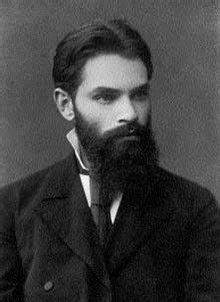
\includegraphics[scale = 0.6]{img/Lyapunov.jpg}
	\caption{}
\end{figure}

李雅普诺夫稳定性理论研究的是在扰动下平衡点的稳定性问题,可以将问题分为以下四种情况(如图\ref{stable}所示):
\par \textbf{$\mathit{1.}$}
如果平衡状态$\bv{x_e}$受到扰动后,仍然\textbf{停留在$\bv{x_e}$附近},我们就称
$\bv{x_e}$在\textbf{李雅普诺夫意义下是稳定的}(Lyapunov stable);

\textbf{$\mathit{2.}$}
如果平衡状态$\bv{x_e}$受到扰动后,\textbf{最终都会收敛到}$\bv{x_e}$,我们就称
$\bv{x_e}$在李雅普诺夫意义下是\textbf{渐进稳定的}(Asymptotically stable);

\textbf{$\mathit{3.}$}
如果平衡状态$\bv{x_e}$受到\textbf{任何扰动}后,\textbf{最终都会收敛到}$\bv{x_e}$,我们就称
$\bv{x_e}$在李雅普诺夫意义下是\textbf{大范围内渐进稳定的}(Asymptotically stable in large);

\textbf{$\mathit{4.}$}
如果平衡状态$\bv{x_e}$受到\textbf{某种扰动}后,\textbf{状态开始偏离}$\bv{x_e}$,
我们就称$\bv{x_e}$在李雅普诺夫意义下是\textbf{不稳定的}(Unstable)。

\begin{figure}[h]
	\centering
	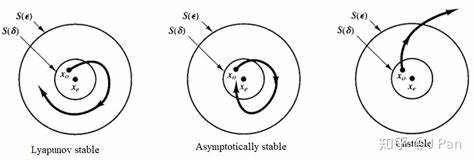
\includegraphics[scale = 0.8]{img/stable.jpg}
	\caption{Lyapunov Stability}
	\label{stable}
\end{figure}

\subsection*{李雅普诺夫第二法}
第二法比较天才,来源于一个朴素的想法:稳定的系统能量总是不断被耗散的,
李雅普诺夫通过定义一个标量函数$V(\bv{x})$(通常能代表广义能量)来分析稳定性。
这种方法的避免了直接求解方程,也没有进行近似线性化,所以也一般称之为直接法。
\begin{theorem}
	如果标量函数$V(\bv{x})$满足:
	\begin{equation*}
		\begin{aligned}
			\bullet ~ & V\left( \boldsymbol{x} \right) =0\,\,\text{if\,\,and\,\,only\,\,if\,\,}\boldsymbol{x}=0                                                                                                    \\
			\bullet ~ & V\left( \boldsymbol{x} \right) >0\,\,\text{if\,\,and\,\,only\,\,if\,\,}\boldsymbol{x}\neq 0                                                                                                \\
			\bullet ~ & \dot{V}\left( \boldsymbol{x} \right) =\frac{d}{dt}V\left( \boldsymbol{x} \right) =\sum_{i=1}^n{\frac{\partial V}{\partial x_i}}f_i\left( x \right) \leq 0~\text{when~}\boldsymbol{x}\neq 0 \\
		\end{aligned}
	\end{equation*}
	\par 则称系统在李雅普诺夫意义下是稳定的,特别的,若$\bv{x} \neq 0$时,有$\dot{V}(\bv{x}) < 0$,
	则系统是渐进稳定的。
\end{theorem}

\par 本节主要参考了\href{https://zhuanlan.zhihu.com/p/58738073}{如何理解李雅普诺夫稳定性分析}

\section{Exponentially Stable}
\begin{definition}[Exponentially Stable]
	假设稳定点$\bv{x^{*}} = 0$为Exponentially Stable平衡点,那么满足存在两个正数k和$\lambda$,$D=\{\bv{x}\in R^n|\|\bv{x}\|<r\}$,$\forall t \geq t_0$,$\forall \bv{x}(t_0) \in D$,使得
	\begin{equation}
		\|\bv{x}(t)\|\leq k\|\bv{x}(t_0)\|e^{-\lambda(t-t_0)}
	\end{equation}
	其中$\lambda$为指数收敛率,k为超调量。
\end{definition}

\begin{theorem}
	假设$\bv{x} = 0$为非线性系统$\dot{\bv{x}}=f(\bv{x})$的平衡点,且$f(\bv{x})$在$\bv{x} = 0$的邻域是连续可微的。令
	\begin{equation}
		A=\left.\frac{\partial f}{\partial \bv{x}}\right|_{\bv{x}=0}
	\end{equation}
	当且仅当A是Hurwitz Matrix(见定义\ref{de1.5})时,$\bv{x}=0$为非线性系统的Exponentially Stable平衡点。
\end{theorem}

\begin{theorem}[Exponential stability theorem]
	假设$\bv{x} = 0$为非线性系统$\dot{\bv{x}}=f(\bv{x},t)$的Exponentially Stable平衡点,$\forall t \geq t_0$,$\forall \bv{x}(t_0) \in D$,
	存在函数V满足以下不等式:
	\begin{equation}
		\begin{aligned}
			 & c_{1}\|\bv{x}\|^{2}\leq V(t,\bv{x})\leq c_{2}\|\bv{x}\|^{2}                                         \\
			 & \frac{\partial V}{\partial t}+\frac{\partial V}{\partial \bv{x}}f(t,\bv{x})\leq-c_{3}\|\bv{x}\|^{2} \\
			 & \left\|{\frac{\partial V}{\partial \bv{x}}}\right\|\leq c_{4}\|\bv{x}\|
		\end{aligned}
	\end{equation}
	\par 其中$c_1,c_2,c_3,c_4,$为正常数。
\end{theorem}

\section{Gronwall-Bellman Inequality}
\begin{theorem}[Gronwall-Bellman Inequality]
	设$I=[a,b]$,$\alpha,\beta,u$为I上的实值函数,$\alpha,u$是I上的连续函数,$\beta$是
	非负的。如果u满足
	\begin{equation}\label{eq3.4}
		u(t)\leq\alpha(t)+\int_a^t\beta(s)u(s)\mathrm{d}s,\quad\forall t\in I
	\end{equation}
	那么
	\begin{equation}\label{eq3.5}
		u(t)\leq\alpha(t)+\int_a^t\alpha(s)\beta(s)\exp\left(\int_s^t\beta(r)\mathrm{d}r\right)\mathrm{d}s,\quad t\in I
	\end{equation}
	如果$\alpha$是非递减函数,我们可以得到
	\begin{equation}\label{eq3.6}
		u(t)\leq\alpha(t)\exp\left(\int_{a}^{t}\beta(s)\mathrm{d}s\right),\quad t\in I
	\end{equation}
\end{theorem}

\begin{proof}
	我们定义一个函数
	\begin{equation}\label{eq3.7}
		v(s)=\exp\left(-\int_a^s\beta(r)\mathrm{d}r\right)\int_a^s\beta(r)u(r)\mathrm{d}r,\quad s\in I
	\end{equation}
	求导,得
	\begin{equation}
		v'(s)=\left(\underbrace{u(s)-\int_a^s\beta(r)u(r)}_{\leq\alpha(s)}\right)\beta(s)\exp\left(-\int_a^s\beta(r)\mathrm{d}r\right),\quad s\in I
	\end{equation}
	积分,得
	\begin{equation}
		v(t)\leq\int_a^t\alpha(s)\beta(s)\exp\left(-\int_a^s\beta(r)\mathrm{d}r\right)\mathrm{d}s
	\end{equation}
	再根据式\ref{eq3.7},得
	\begin{equation}\label{eq3.10}
		\begin{aligned}
			\int_{a}^{t}\beta(s)u(s)\mathrm{d}s
			 & =\exp\left(\int_a^t\beta(r)\mathrm{d}r\right)v(t)                                                                                                            \\
			 & \leq\int_a^t\alpha(s)\beta(s)\exp\left(\underbrace{\int_a^t\beta(r)\mathrm{d}r-\int_a^s\beta(r)\mathrm{d}r}_{=\int_s^t\beta(r)\mathrm{d}r}\right)\mathrm{d}s
		\end{aligned}
	\end{equation}
	把式\ref{eq3.10}带入式\ref{eq3.4},即得式\ref{eq3.5}。

	再根据$\alpha$为非递减函数,我们可以得到$\alpha(s)\leq \alpha(t)$,带入式\ref{eq3.5},即得
	\begin{equation*}
		\begin{gathered}
			u(t)
			\leq\left.\alpha(t)+\left(-\alpha(t)\exp\left(\int_s^t\beta(r)\mathrm{d}r\right)\right)\right|_{s=a}^{s=t} \\
			=\alpha(t)\exp\left(\int_{a}^{t}\beta(r)\mathrm{d}r\right),\quad t\in I.
		\end{gathered}
	\end{equation*}
	即证式\ref{eq3.6}。

	证毕!

\end{proof}

\chapter{Calculus}
\section{矩阵与范数求导}

\subsection{梯度}

\begin{theorem}
	假设$\mathbf{x}$为$n$维向量,在微分多元函数时经常使用以下规则:
	\begin{enumerate}[1、]
		\item     对于所有$\mathbf{A} \in \mathbb{R}^{m \times n}$,都有$\nabla_{\mathbf{x}} \mathbf{A} \mathbf{x} = \mathbf{A}^\top$
		\item 对于所有$\mathbf{A} \in \mathbb{R}^{n \times m}$,都有$\nabla_{\mathbf{x}} \mathbf{x}^\top \mathbf{A}  = \mathbf{A}$
		\item 对于所有$\mathbf{A} \in \mathbb{R}^{n \times n}$,都有$\nabla_{\mathbf{x}} \mathbf{x}^\top \mathbf{A} \mathbf{x}  = (\mathbf{A} + \mathbf{A}^\top)\mathbf{x}$
		\item $\nabla_{\mathbf{x}} \|\mathbf{x} \|^2 = \nabla_{\mathbf{x}} \mathbf{x}^\top \mathbf{x} = 2\mathbf{x}$
	\end{enumerate}
\end{theorem}

同样,对于任何矩阵$\mathbf{X}$,都有$\nabla_{\mathbf{X}} \|\mathbf{X} \|_F^2 = 2\mathbf{X}$。
正如我们之后将看到的,梯度对于设计深度学习中的优化算法有很大用处。

\subsection{矩阵微分}
\begin{corollary}
	假设$\mathbf{x}$是t的函数,则
	\begin{equation}
		\frac{d(\mathbf{x}^TA\mathbf{x})}{dt} = (d\mathbf{x})^TA\mathbf{x} + \mathbf{x}^TA(d\mathbf{x})
	\end{equation}
\end{corollary}



\section{向量函数的$Taylor$公式}\label{eq4.1}
对于向量$\bv{x,x_0}$和标量函数$f(\bv{x})$,我们有
\begin{equation}
	f(\bv{x}) = f(\bv{x_0}) + (\bv{x-x_0})^T\nabla f(\bv{x_0}) + \cdots
\end{equation}





\chapter{Game Theorem}



\chapter{Advanced Algebra}
\section{Gerschgorin Circle Theorem—特征值估计\label{Gerschgorin}}
\begin{theorem}[圆盘第一定理]\label{Gerschgorin1}
	设A是n阶复矩阵,$A=(a_{ij})_{n \times n}$,则A的特征值在复平面上的下列圆盘(又称戈式圆盘)中:
	\begin{equation*}
		|z-a_{ii}|\leq R_i,i=1,2,\ldots,n
	\end{equation*}
	\par 其中$R_i$为A的第i行元素去掉$a_{ii}$后的绝对值之和,即
	\begin{equation*}
		R_i=\sum_{j\neq i}^n|a_{ij}|=|a_{i1}|+\cdots+|a_{i,i-1}|+|a_{i,i+1}|+\cdots+|a_{in}|
	\end{equation*}
\end{theorem}

\begin{lemma}
	设\begin{equation*}
		f(x)=a_nx^n+a_{n-1}x^{n-1}+\cdots+a_1x+a_0
	\end{equation*}
	\par 是n次复系数多项式,则$f(x)$的n个根$\lambda_{1},\lambda_{2},\ldots,\lambda_{n}$都是$a_n,a_{n-1},\ldots a_1,a_0$
	的连续函数。
\end{lemma}

\begin{theorem}[圆盘第二定理]
	设矩阵$A=(a_{ij})_{n \times n}$的n戈氏圆盘分成若干个连通区域,若其中一个连通区域含有
	k个戈氏圆盘,则有且只有k个特征值落在这个连通区域内(若两个戈氏圆盘重合,需计重数;又若特征值为重根,也计重数)。
\end{theorem}

本节主要参考了\href{https://zhuanlan.zhihu.com/p/418915975}{特征值的估计——圆盘定理(Gerschgorin(戈氏)圆盘第一定理)}
和\href{https://zhuanlan.zhihu.com/p/419195345}{特征值的估计——圆盘定理(Gerschgorin(戈氏)圆盘第二定理)},
在文章中会有具体的证明。

\section{Jordan Form}
\begin{definition}[Jordan Form]
	矩阵$J$除了主对角线和主对角线上方元素之外,其余都是0,且主对角线上方的对角线的系数若不为0只能为1
	。且这1的左方和下方的系数(都在主对角线上)有相同的值。
	\begin{equation}
		J=\operatorname{Diag}(J_1,J_2,\ldots,J_r)=
		\left(\begin{array}{cccc}
				\boxed{J_1} & 0           & \ldots & 0           \\
				0           & \boxed{J_2} & \ddots & \vdots      \\
				\vdots      & \ddots      & \ddots & 0           \\
				0           & \ldots      & 0      & \boxed{J_r}
			\end{array}\right)
	\end{equation}
	\par 其中$J_1,J_2,\ldots,J_r$为Jordan Block。易知对角矩阵是一种特殊的Jordan标准型矩阵。
\end{definition}
\begin{definition}[Jordan Block]
	形如矩阵$J\left(\lambda,t\right)$的形式被称为Jordan Block。
	\begin{equation}
		J\left(\lambda,t\right)=
		\begin{pmatrix}
			\lambda & 0       & \cdots & 0      & 0       & 0       \\
			1       & \lambda & \cdots & 0      & 0       & 0       \\
			\vdots  & \vdots  & \vdots & \vdots & \vdots  & \vdots  \\
			0       & 0       & \cdots & 1      & \lambda & 0       \\
			0       & 0       & \cdots & 0      & 1       & \lambda
		\end{pmatrix}_{(t\times t)}
	\end{equation}
\end{definition}
\begin{example}
	对于矩阵J,它的Jordan Block为$\begin{bmatrix} 1 \end{bmatrix}$,$\begin{bmatrix} 2 \end{bmatrix}$,
	$\begin{bmatrix} 4&1\\0&4\end{bmatrix}$。
	\begin{equation*}
		J=
		\begin{bmatrix}
			1 & 0 & 0 & 0 \\
			0 & 2 & 0 & 0 \\
			0 & 0 & 4 & 1 \\
			0 & 0 & 0 & 4
		\end{bmatrix}
	\end{equation*}
\end{example}

\section{矩阵特征值不等式}
\begin{theorem}
	对于任意向量$\bv{x}$和实对称矩阵$A$,我们有
	\begin{equation}
		\lambda_{\mathrm{min}}\left(A\right)\leq\frac{x^{T}Ax}{x^{T}x}\leq\lambda_{\mathrm{max}}\left(A\right)
	\end{equation}
\end{theorem}
\begin{proof}
	存在正交矩阵$T$,满足
	\begin{equation*}
		T^TAT = \begin{pmatrix}
			\lambda_1 &           &        &           \\
			          & \lambda_2 &        &           \\
			          &           & \ddots &           \\
			          &           &        & \lambda_n
		\end{pmatrix}
	\end{equation*}
	令$\bv{x} = T\bv{y}$,我们可以得到
	\begin{equation*}
		\frac{x^{T}Ax}{x^{T}x}=\frac{y^{T}\left(
			\begin{matrix}\lambda_{1} &             &        & \\
                          & \lambda_{2} &        & \\
                          &             & \ddots & \\&&&\lambda_{n}
				\end{matrix}\right)y}{y^{T}y}
		=\frac{\lambda_{1}y_{1}^{2}+\lambda_{2}y_{2}^{2}+\cdots+\lambda_{n}y_{n}^{2}}{y_{1}^{2}+{y}_{2}^{2}+\cdots+{y}_{n}^{2}}
	\end{equation*}
	放缩,即得
	\begin{equation*}
		\lambda_{min}(A)\frac{y_{1}^{2}+y_{2}^{2}+\cdots+y_{n}^{2}}{y_{1}^{2}+y_{2}^{2}+\cdots+y_{n}^{2}}
		\leq \frac{x^{T}Ax}{x^{T}x}
		\leq \lambda_{max}(A)\frac{y_{1}^{2}+y_{2}^{2}+\cdots+y_{n}^{2}}{y_{1}^{2}+y_{2}^{2}+\cdots+y_{n}^{2}}
	\end{equation*}
	证毕!
\end{proof}







\appendix

\chapter{[1]Distributed Nash Equilibrium Seeking by a Consensus Based Approach}
\section{Terminology}
\begin{enumerate}
	\item penetration:n.渗透
	\item exploit:vt.利用
	\item utilize:vt.利用
	\item asynchronous:adj.异步的
	\item payoff:n.收益
	\item saddle poiont:n.鞍点
	\item permutation:n.排列
	\item consensus:n.一致
	\item protocol:n.协议
	\item collaboratively:adv.合作的
	\item convergence:n.收敛
	\item adoption:n.采用
	\item successively:n.相继的
	\item auxiliary:adj.辅助的
\end{enumerate}

\section{式(8)中的Hurwitz Matrix}
试证明$-(L\otimes I_{N\times N}+B_{0})$是Hurwitz Matrix
\begin{proof}
	对角线上的元素为$-a_{i}-\sum_{j=1}^{N}a_{ij},半径R_i = \sum_{j=1}^{N}|a_{ij}|$,根据定理\ref{Gerschgorin1},我们可以得到
	\begin{equation*}
		\lambda_i \leq -a_{i}-\sum_{j=1}^{N}a_{ij} + R_i = -a_{i}\leq 0
	\end{equation*}
	特征值都小于等于0,故其为Hurwitz Matrix。
\end{proof}





\section{线性化式(19)}
我们取$\bv{x-x_0} \rightarrow 0$,根据公式\ref{eq4.1},我们有
\begin{equation*}
	\begin{aligned}
		\frac{\partial f_i(\bv{x})}{\partial x_i} & = \frac{\partial f_i(\bv{x^{*}})}{\partial x_i} +
		(\bv{x-x^{*}})^T(\frac{\partial \frac{\partial f_i(\bv{x^{*}})}{\partial x_i}}{\partial \bv{x}}) \\
		                                          & =
		(\bv{x-x^{*}})^T(\frac{\partial \frac{\partial f_i(\bv{x^{*}})}{\partial x_i}}{\partial \bv{x}})
	\end{aligned}
\end{equation*}

证毕!


\section{式(20)中\texorpdfstring{$\overline{\bv{k}} B$}{防缺字}is Hurwitz}
根据定理\ref{Gerschgorin1},我们知道
\begin{equation*}
	|\lambda_i - \frac{\partial^2f_i}{\partial x_i^2}| \leq R_i
\end{equation*}
即
\begin{equation*}
	\frac{\partial^2f_i}{\partial x_i^2} - R_i \leq \lambda_i \leq \frac{\partial^2f_i}{\partial x_i^2} + R_i
\end{equation*}
而
\begin{equation*}
	|\frac{\partial^2f_i}{\partial x_i^2}| > |R_i|,\frac{\partial^2f_i}{\partial x_i^2} < 0
\end{equation*}
所以$\lambda_i < 0$,$i = 1, 2,\ldots,N$,证毕!




\end{document}
